
\subsection{Image to Latex}
Given images captured via airdrawing, a transformer encoder-decoder network is used to translate the images to \LaTeX\ . The VTex network borrows much of its ideas from the Bidirectionally Trained Transformer (BTTR) without adopting the bidirectional training strategy \cite{ZhaoBTTR2021}. The model is implemented from scratch in PyTorch using the architecture shown in Figure \ref{fig:architecture}.

\begin{figure}[h!]
    \centering
    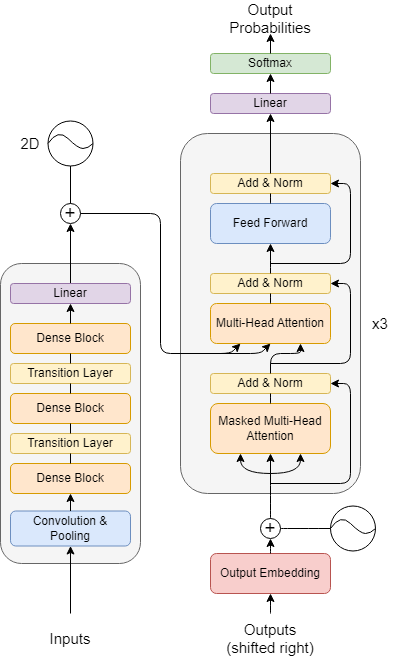
\includegraphics[width=7cm]{images/vtex_network.png}
    \caption{Architecture of the VTex translation network}
    \label{fig:architecture}
\end{figure}

\subsubsection{Decoder}
The decoder is constructed in the same manner as the original transformer paper \cite{Attention}. First, the decoder input is embedded to convert the target sequence to a $d_{model}$ dimension vector. Then, positional encoding is added in the manner described in Section \ref{sec:positionalencoding}. This is then fed into the decoder layers. 

Each decoder layer consists of three sublayers: a masked multi-head attention module that performs self-attention on the decoder input, a multi-head attention module that performs attention on the encoder output, and a feed-forward network. Residual connections and layer norms are appended to each sublayer. 

The multi-head attention modules utilize "Scaled Dot-Product Attention" as described in \cite{Attention}. This attention mechanism matches a set of queries to key-value pairs. Given a set of queries $Q$, keys $K$, and values $V$, the attention can be computed as:

\begin{equation} \label{eq:scaledattention}
\begin{split}
    \textrm{Attention}(Q,K,V) = \textrm{softmax}(\frac{QK^T}{\sqrt{d_k}}V)
\end{split}
\end{equation}

Furthermore, multi-head attention splits $Q,K,$ and $V$ into $h$ different heads with $d_{model}/h=d_k$ dimension vectors, performing the attention computation shown in Equation \ref{eq:scaledattention} on each head in parallel. The heads are then concatenated for the final attention values. Thus,

\begin{equation} \label{eq:multihead}
\begin{split}
    \textrm{MultiHead}(Q,K,V) = \textrm{Concat}(\textrm{head}_1, \textrm{...},\textrm{head}_h)W^O \\ 
    \textrm{ where head}_i = \textrm{Attention}(QW_i^Q, KW_i^K, VW_i^V)
\end{split}
\end{equation}
where $W^O, W_i^Q, W_i^K, W_i^V$ are projection matrices that reshape the vector dimensions to $d_{model}, d_k, d_k, d_k$ dimensions, respectively. 


As the decoder input (Output Embedding in Figure \ref{fig:architecture}) contains the full target sequence at each time step, it is imperative for training that tokens do not pay attention to future tokens, as this does not reflect how the model will perform in practice. As such, the decoder input is masked such that tokens can only pay attention to past tokens and the input image.

The second multi-head attention module utilizes the first attention module's output as the queries and the encoder's output as the keys and values. Finally, this output is fed into the feed-forward layer, which expands the $d_{model}$ dimension vector to dimension $d_{ff}$ and back to $d_{model}$.

The VTex decoder consists of 3 decoder layers, each with $h=8$ heads, model dimension $d_{model}=256$, feed-forward inner layer dimension $d_{ff}=1024$, and dropout rate of $0.3$.

\subsubsection{Encoder}
The original transformer fails when we introduce images as the source input. Applying self attention to every pixel in an image is far too demanding for modern hardware. As such, image analysis is often done by convolutional neural networks (CNN). For the purposes of encoding, a CNN performs well in feature extraction and classification problems. VTex uses the DenseNet architecture to extract information at multiple scales of the mathematical symbols present in an image \cite{Densenet2017}.

DenseNet is based on the concept of "dense connectivity," meaning each layer in the network is connected to every other layer in a feed-forward fashion. Doing so promotes gradient propagation, allowing the network to learn features at all complexity levels. This allows DenseNet to outperform other CNNs when training data is limited, and this is why VTex uses it. Specifically, VTex uses the DenseNet-B model noted in \cite{Densenet2017}, which adds "bottleneck" layers (i.e. 1x1 convolutions) to reduce input features and improve computational efficiency. Finally, a 1x1 convolution is applied to reshape the DenseNet output to fit the decoder.

While a traditional DenseNet is extremely prone to overfitting, VTex greatly simplifies the model by using .bmp binary images. As for the hyperparameters, this paper's implementation uses 3 bottleneck dense blocks with a growth rate of $k=24$, block depth of 16, and compression factor of $\theta = 0.5$.

\subsubsection{Positional Encoding} \label{sec:positionalencoding}
In a traditional transformer, the decoder must use a positional encoding to embed sequence ordering or tokens. VTex adopts the sinusoidal positional encoding presented in the original transformer for this purpose \cite{Attention}.
For a $d$ dimension encoding, the positional encoding can be defined as:

\begin{equation} \label{eq:wordposenc}
\begin{split}
PE_{(pos, 2i, d)} = \sin(pos/10000^{2i/d}) \\
PE_{(pos, 2i+1, d)} = \cos(pos/10000^{2i/d})
\end{split}
\end{equation}

where $pos$ is the position of the token and $i$ is the dimension index. This positional encoding is added to the target output before any decoder layers.

In encoding an image, the encoder must account for both a symbol's classification and the symbol's relationship with other symbol (e.g. within the same fraction, in a superscript, etc.). These relationships often cannot be extracted using only a simple CNN. While others have used graph neural networks to learn these relationships \cite{Peng2021}, VTex's encoder models these relationships as positional encodings much like the decoder does. Specifically, Equation \ref{eq:wordposenc} is applied in both the height and width axes of the input image such that for a pixel $(x,y)$:

\begin{equation} \label{eq:imgposenc}
\begin{split}
PE_{((x, y), 2i, d)} = [ PE_{(x, 2i, d/2)} ; PE_{(y,2i,d/2)} ] \\
PE_{((x, y), 2i+1, d)} = [ PE_{(x, 2i+1,d/2)} ; PE_{(y,2i+1,d/2)} ]
\end{split}
\end{equation}

In the encoder, the positional encoding is added to the CNN output before being fed into the decoder.

\subsubsection{Prediction Step}
Because the output of a transformer is the next token in a sequence, the search space grows exponentially with the sequence length. Performing an exhaustive search for every image is impractical with modern hardware. Often, inferencing with a transformer is a balance between accuracy and computational efficiency. In this paper, two prediction methods are implemented to infer an output sequence from an image. 

A greedy approach starts with a {\tt <SOS>} (start of sequence) token and predicts the most probable next token, iteratively adding the output token to the input sequence until the transformer predicts a {\tt <EOS>} (end of sequence) token. This is the simplest approach to inferencing with a transformer. However, there are cases where a less probable token will become more probable as the transformer uncovers more of the sequence. For example, at time step 1, a transformer will predict the first token as $x$, but later at time step 5, the transformer will realize that the first token should be $y$. In this manner, a single wrong classification will disrupt the rest of the output sequence.

A beam search approach remedies this problem by exploring multiple possible predictions, i.e. "beams", for each time step. With a beam size of $k$, the top $k$ sequences across all time steps will be considered for the decoder input. In addition, longer sequences will be penalized to prevent the inferencing from never ending. Inferencing terminates when all beams contain a {\tt <EOS>} token. Then, the most probable beam is chosen as the final output sequence.

This paper implements beam search with size $10$. The results using greedy vs. beam search are discussed in Section \ref{sec:eval}. 


\subsection{Data Collection} \label{sec:datacollection}
Two datasets were considered for training the model. The public {\tt IM2LATEX-100K} dataset provides 103,556 pairs of \LaTeX\ equations with pictures of their rendered images \cite{im2latex}. The large size of this dataset makes it a prime candidate for training a complex neural network like VTex. However, its rendered images are of printed text--not handwritten equations. As such, it may not perform well when paired with the virtual drawing component of the VTex pipeline. To remedy this, transfer learning can be applied using a handwritten math symbols dataset, fine-tuning the CNN encoder \cite{HandwrittenMath}.

Alternatively, the Competition on Recognition of Handwritten Mathematical Expressions (CROHME) provides a dataset of 8836 training images of handwritten mathematical expressions \cite{CROHME}. CROHME does not provide data in the format VTex desires. Rather, the input is an InkML or Label Graph (LG) file that represents strokes captured by a tablet, and the output is a tree-based symbolic representation named Symbol Layout Graph (symLG). Fortunately, CROHME provides tools to convert these file types into images (.bmp) and \LaTeX\ code, respectively, shown in Figure \ref{fig:datasample}. As VTex's final goal is to process handwritten equations, the CROHME dataset was chosen despite its smaller size. This would present challenges as documented in Section \ref{sec:results}. The CROHME 2014 test set, containing 986 images, is used as the validation set.

\begin{figure}[h!]
    \centering
    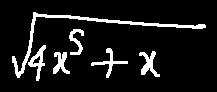
\includegraphics{images/20_em_40.png}
    \begin{verbatim}
        \sqrt { 4 x ^ { 5 } + x }
    \end{verbatim}
    \caption{Example converted .bmp image with its ground truth from the CROHME training set}
    \label{fig:datasample}
\end{figure}

